\documentclass[a4paper,11pt]{article}
\usepackage{fullpage}
\usepackage{graphicx}
\usepackage{eqnarray,amsmath, amssymb}
\usepackage{bookmark}
\usepackage{hyperref}

\usepackage{listings}
\usepackage{changepage}

\makeatletter
\renewcommand\@seccntformat[1]{}
\makeatother
\hypersetup{pdfinfo={
Title = {ELEN3007-Assignment-2024},
Author = {Kgadile "Naar-Kie" Masemola},
CreationDate = {D:202409120836},
%ModDate = {D:202409040530},
Subject = {ELEN3XXX Paper Format, 2024}
%/Keywords (ELEN3007, naar_kie, paper, project)
}}

%%%%%%%%%%%%%%%%%%%%%%%%%%%%%%%%%%%%%%%%%%%%%%%%%%%%%%%%%%%%%%%%%%%%%%%%%%%%%%%%%%%%%%%%%%%%

\title{ELEN3007A Group \underline{27} - Assignment 2024: \\ 
\large \emph{Application of Bayes’ Theorem for Locating a Robot’s
Position in an Enclosed Area}}
\author{Kgadile E Masemola (876729)}
\date{September 13, 2024}

\begin{document}
\maketitle

\section{QUESTION 1:}  Why does $\theta_k$ not lie between $- \pi$ and $\pi$ for which $p(\theta_k | \alpha, \beta, B)$ would then be $\frac{1}{2\pi}$?

\subsection*{\underline{Solution 1:}}
The setup of the problem indicates that the photodetectors are placed along the x-axis, above
which the robot is located. Therefore, the signal originates from one side of the horizontal axis.
This limits the range of the detectors to capture only collimated flashes within the azimuth $-\frac{\pi}{2}$ to $\frac{\pi}{2}$. . 

\section{QUESTION 2:}
Prove that
\begin{equation}
	p(x_k | \alpha, \beta, B) = \frac{\beta}{\pi (\beta^2 + (x_k - \alpha)^2)}
\end{equation}
\subsection*{\underline{Solution 2:}}
\label{sec:proof}
Using the relation $x_k = \alpha + \beta \tan \theta_k$ (given in the brief \cite{vanWyk2024}) and the prior PDF $p(\theta_k | \alpha, \beta, B) = f_{\Theta | \Lambda, \beta, B}(\cdot) = \frac{1}{\pi}$. Then we apply transformation of random variables (notations for random variables defined \hyperref[sec:notation]{\textbf{Solution 8}}). The change of variables  $x = g(y) \Rightarrow \theta_k = g(x_k)$. The function $f(\theta)$ becomes $\tilde{f} = f(g(x))$. The given PDF $f_\Theta (\theta)$ corresponds to $f_X (x)$ with respect to new variable $x$. Therefore change of variables for PDF's equation, adapted from \cite{bishop2006pattern}, leads to the PDF transformation as:
\begin{equation}
	p_x(x) = p_\theta(\theta) \left| \frac{d\theta}{dx} \right| = p_\theta (g(x))|g^,(x)|
\end{equation}
using the correct notation and given $x_k$ relation:
\begin{align}
	f_X(x_k) &= f_\Theta (\theta_k) \times \left| \frac{d\theta_k}{dx_k} \right| = f_\Theta (\theta_k) \times \left| \left(\frac{dx_k}{d\theta_k} \right)^{-1} \right| \\
	&= \frac{1}{\pi} \times \left| \left( \frac{d}{d\theta_k}(\beta \tan \theta_k + \alpha) \right)^{-1}  \right| =\frac{1}{\pi} \times \left| \frac{1}{\beta \sec^2\theta_k} \right| \nonumber\\
	but \; \sec^2(\theta_k) &= 1 + \tan^2\theta_k \; and \; \tan\theta_k = \frac{x_k - \alpha}{\beta} \; (relation)\\
	so \; &= 1 + \left(\frac{x_k - \alpha}{\beta} \right)^2 = \frac{\beta^2 + (x_k - \alpha)^2}{\beta^2} \nonumber
\end{align}
	
\begin{align}
	\therefore \; f_X(x_k) &= \frac{1}{\pi} \times \frac{\beta^2}{\beta(\beta^2 + (x_k - \alpha)^2}\\
	and, \; so \; f_X(x_k) &\leftrightharpoons f_{X | \Lambda, \mathfrak{B}, B}(\, \cdot \, | \alpha, \beta) \; and \; f_\Theta (\theta_k) \leftrightharpoons f_{\Theta | \Lambda, \beta, B}(\cdot) \nonumber\\
	thus \; f_{X | \Lambda, \mathfrak{B}, B}(\, \cdot \, | \alpha, \beta) &= \frac{\beta}{\pi (\beta^2 + (x_k - \alpha)^2)} \; \blacksquare
\end{align}

\section{QUESTION 3:}
Plot $p(x_k | \alpha, \beta, B)$ and then relate its width at half maximum to the parameters of the PDF.

\subsection*{\underline{Solution 3:}}
The plot of the PDF $ p(x_k | \alpha, \beta, B) \Rightarrow f_{X | \Lambda, \mathfrak{B}, B}(x_k |\Lambda = \alpha, \mathfrak{B} = \beta)$ is shown in Figure 1 below. The \emph{parameters} are chosen to be $\alpha = 4; \beta = 2$ for $\{x_k \}^ {10} _{k = -10}$. It shows that the maximum peak value is when $x_k = 4 = \alpha$. At half maximum of \emph{these} paramaters, the width of the distribution is $4 = 2 \beta$, half maximum height is $y = 0.1591536$.

\begin{figure}[h]
        \centering
        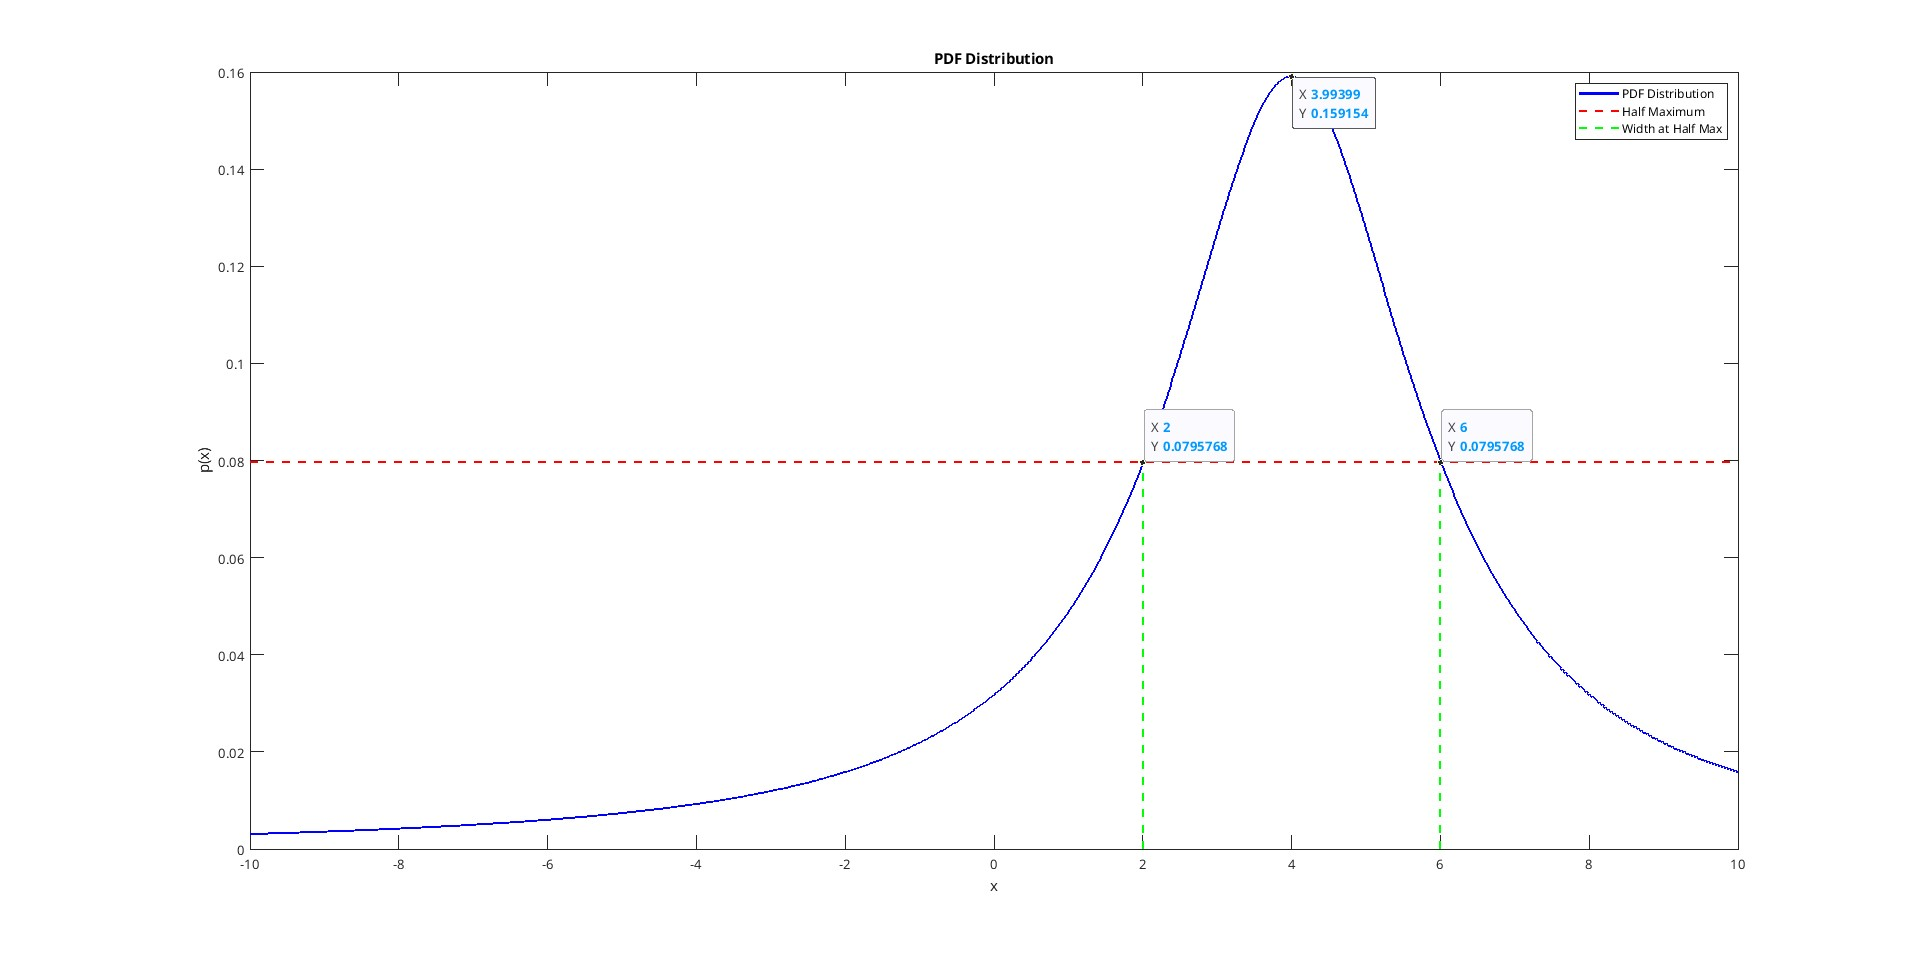
\includegraphics[scale=0.16]{q03pdfplot.jpg} 
        \caption{Q3 Plot of the PDF $p(x_k | \alpha, \beta, B)$}
\end{figure}


\section{QUESTION 4:}
Derive the expression for $p(\alpha | x_k, \beta, B)$.

\subsection*{\underline{Solution 4:}}
The conditional distribution of $\Lambda(\cdot)$ \underline{given} $X(\cdot), \, \mathfrak{B}(\cdot)$, Bayes' Theorem requires equation (7) \emph{(notation in \hyperref[sec:notation]{\textbf{Solution 8}})}, from \cite{stanford_lecture20}:
\begin{equation}
	f_{\Lambda | X, \mathfrak{B},B} (\, \cdot \, | x_k, \beta) = \frac{f_{X | \Lambda, \mathfrak{B},B}(\, \cdot \, | x_k, \beta)}{f_X(x_k)} =
	\frac{f_{X | \Lambda, \mathfrak{B},B}(\, \cdot \, | x_k, \beta) f_\Lambda(\cdot)}{f_X(x_k)}
\end{equation}
But, we can similarly use the same method as proof in \hyperref[sec:proof]{\textbf{Solution 2}} by setting $\alpha$ as the subject of the formula in the relation $\Rightarrow \alpha = -(\beta \tan \theta_k - x_k)$. We get:

\begin{align}
	f_{\Lambda | X, \mathfrak{B},B} (\, \cdot \, | x_k, \beta) &= f_\Theta (\theta_k) \times \left| \frac{d\theta_k}{d\alpha} \right| = f_\Theta (\theta_k) \times \left| \left(\frac{d\alpha}{d\theta_k} \right)^{-1} \right| \\
	but, \; \frac{d\alpha}{d\theta} &= -\beta \sec^2 \theta_k \; \Rightarrow \; \left| \left(\frac{d\alpha}{d\theta_k} \right)^{-1} \right| = \frac{1}{\beta \sec^2 \theta_k}
\end{align}
as above, substituting (9) in (8) and $f_\Theta (\theta_k) = \frac{1}{\pi}$, and using \hyperref[sec:proof]{\textbf{2}}, we get still get:
\begin{equation}
	f_{\Lambda | X, \mathfrak{B},B} (\, \cdot \, | x_k, \beta) = \frac{1}{\pi} \frac{\beta}{(\beta^2 + (x_k - \alpha)^2)} \; \blacksquare
\end{equation}

\section{QUESTION 5:}
Finally derive an expression for $p(\alpha | \{x_k\}^N _{k = 1}, \beta, B)$. (State all assumptions.)

\subsection*{\underline{Solution 5:}}
Assumptions:
\begin{itemize}
	\item The prior PDF is given as $f_{\Theta|\Lambda, \mathfrak{B},B}(\cdot) = \frac{1}{\pi}$. And using the transformation of random variables in \hyperref[sec:proof]{\textbf{2}} , becomes $f_{X | \Lambda, \mathfrak{B}, B}(\, \cdot \, | \alpha, \beta)$ equation (6).
	\item The measurements $\{x_k\}^N _{k = 1}$ are input to the random variable $X_k(\cdot) = \{x_k\}^N _{k = 1}$.
	\item $\{x_k\}^N _{k = 1}$ are independent, and continuous.. thus $X_k(\cdot)$ is a continuous. random variable.
	\item The normalisation(/marginal probability of observed data/ proportionality factor) $f_X(x_k) \approx weird \; integral \backsimeq constant$ in eqaution (7) is discarded $\because$ it does not depend on $\alpha$. It is just a scalling factor which doesn't affect the peak point $\alpha$. 
	\item So we can use the \emph{Posterior density $\varpropto$ Likelyhood $\times$ Prior Density} \cite{stanford_lecture20}, where the individual distributions can be inferred from (10):
		\begin{equation}
			f_{\Lambda | X, \mathfrak{B},B} (\, \cdot \, | x_k, \beta) \varpropto f_{X | \Lambda, \mathfrak{B}, B}(\, \cdot \, | \alpha, \beta) f_\Lambda(\alpha)
		\end{equation}
\end{itemize}
Then the joint distribution of $p(\alpha | \{x_k\}^N _{k = 1}, \mathfrak{B}, B)$:
\begin{equation}
	f_{\Lambda | X_k, \mathfrak{B},B} (\alpha | x_1,...,x_N, \beta) = \prod^N _{k = 1} \frac{\beta}{\pi (\beta^2 + (x_k - \alpha)^2)} \times \aleph \; \blacksquare
\end{equation}
$\aleph$ is the proportionality factor which may be ignored.

\section{QUESTION 6:}
Explain how one obtains the $x$-position of the robot from the result in (5.).

\subsection*{\underline{Solution 6:}}
The $x$-position of the robot is determined by taking the product of the distributions of each $x_k$, as shown in equation (12) from the result in (5.). This is due to the fact that the measurements are independent.\\ \\
The $x$-position can also be obtained by locating the peak of the distribution (plot) and mapping it to the random variable variable axis. Additionally another method is to use Maximum-A-Posterior (MAP). We can also estimate the posterior mean by applying maximum likelyhood solution $\mu_{ML}$ to the mean of the data distribution and the mean of the prior distribution $\mu_0$. This way the estimate will be a compromise between $\mu_0$ and $\mu_{ML}$. The more measurements we use, the more the estimate approximate to $\mu_{ML}$.

\section{QUESTION 7:}
Implement the Bayesian position inference scheme in Matlab. Assume the robot is
located inside a confined square region of size $10$m $\times$ $10$m. Demonstrate your Bayes
estimator by inferring the robot’s $x$-position from the data/measurements $\{ x_k \}^{200} _{k = 1}$ in \emph{BayesData.mat}, with the robot’s $y$-position 4.5 m. Plot the Bayes posterior distribution for the first $N = 1, 2, 5$ and $30$ measurements. For this data, what is your best $x$-position estimate?

\subsection*{\underline{Solution 7:}}
The Bayesian position inference scheme MATLAB code is attached in Appendix A. The plots are attached in Appendix B as Figures 2 \& 3. The scheme tests the first $N = 1,\; 2, \; 5, and \; 30$. Case 1 consideres the first points that are detected inside the $10 \times 10$ box. Case 2 does not have restrictions and thus uses the first values.\\ \\
It is noticed that when points are restricted to be inside the box, the estimate $\alpha \approx 5.85$, which is within the box, close the midpoint. However, when all points are considered, the mean estimates $\alpha \approx 10.16$ for $N = 30$. But strangely this is outside the box.
In comparing the distribution for the different $N$-measurements, the distribution peak seems to move, and gets thinner and taller as more measurements are known. \\ \\
Maximum likelihood estimate (MLE) solution was applied to the data $\{ x_k \}^{200} _{k = 1}$. The code is attached in Appendix C. The estimation of $\alpha \approx 7.2287$. Comparing this value to posterior-PDF values inside the box (Figure 2) for N = 2 \& 30, the approximate value of $\alpha$ moves further away from the MLE value as N increases.\\\\
After conducting this assignment, we conclude that: 1) The posterior distribution provides a way to quantify the uncertainty in the robot's position estimate. Instead of providing a single “best guess,” Bayesian inference offers a probabilistic distribution over all possible positions, allowing for a richer representation of uncertainty.; 2) The number of measurements significantly affects the shape of the posterior distribution. The more data we have, the better your estimates; 3) In contrast to maximum likelihood estimation (MLE), which finds the single parameter value that maximizes the likelihood, Bayesian inference provides a full posterior distribution, reflecting a range of possible outcomes.\\ \\
After this analysis, the best estimate of $x$-position, based on posterior inference for points inside the box with $N = 30$, is approximately $\alpha \approx 5.85568$. See Figure 2 in Appendix B. $\blacksquare$

\section{QUESTION 8:}
The notation presented above, deliberately does \emph{not} follow the conventions your Probs
lecturer introduced. Throughout your assignment, strictly use the notation prescribed for
use in Probs.
\subsection*{\underline{Solution 8:}}
\label{sec:notation}
Yes with the following Random Variable Notations and Equations: 
 	\begin{eqnarray}
		\Lambda (\cdot) = \alpha;\: \mathfrak{B}(\cdot) = \beta ; \: X(\cdot) = x_k; \: \Theta ( \cdot) = \theta_k \\		
		p(\theta_k | \alpha, \beta, B) = f_{\Theta | \Lambda, \beta, B}(\, \cdot \, | \alpha, \beta) = f_{\Theta | \Lambda, \beta, B}(\cdot)\\
		p(\alpha | x_k, \beta, B) = f_{\Lambda | X, \mathfrak{B}, B}(\, \cdot \, | x_k, \beta) = f_{\Lambda | X, \mathfrak{B}, B}(\cdot) \\\ 
		p(x_k |\alpha, \beta, B) = f_{X | \Lambda, \mathfrak{B}, B}(\, \cdot \, | \alpha, \beta)
	\end{eqnarray}

\section{QUESTION 9:}
Professional report with clear and effective data representation. The report must not have
a title page and is not allowed to exceed 5 pages in length.
\subsection*{\underline{Solution 9:}}
The report is presented in homework assignment form(statement and solution). Additionally, the following reference materials have been consulted for the assignment: \cite{leon2017probability}, \cite{bishop2006pattern}

\section{(Bonus) QUESTION 10:}
Infer both the $x$-position as well as the $y$-position of the robot. Estimate both $\alpha$ and $\beta$ for the PDF in Eq. (1).
\subsection*{Solution 10:} \emph{(Solution is to be provided.)}



\bibliographystyle{unsrt}
\bibliography{elen3007ref}

\newpage
\appendix

\makeatother
\section{Appendix A. - Matlab Inference Scheme Code}
\begin{lstlisting}[language=Matlab,
                   numbers=left,
                   basicstyle=\footnotesize,
                   stepnumber=1,
                   numbersep=10pt,
                   tabsize=2,
                   showspaces=false,
                   showstringspaces=false]
%%%%%%%%%Bayesian Position Inference Scheme%%%%%%%%%%%%
%numbat24.04%
%
% Main function to execute the Bayesian inference and plot results
function BayesianPositionInferenceScheme()
    load('BayesData.mat');
    % Given beta value and alpha range
    beta = 4.5;
    alpha_values = linspace(-50, 50, 1000);

    % Number of measurements to evaluate the posterior
    N_values = [1, 2, 5, 30];

    % Case 1: Points Inside the Box (0 <= x <= 10)
    x_inside_box = x(x >= 0 & x <= 10);
    plot_posterior(x_inside_box, N_values, alpha_values, beta, ...
        'Posterior for Points Inside the Box (0 <= x <= 10)');

    % Case 2: All Points (No Restrictions)
    x_all_points = x; 
    plot_posterior(x_all_points, N_values, alpha_values, beta, 
    'Posterior for All Points');
end

% Function to calculate the posterior for a given dataset and N points
function posterior_values = calculate_posterior(data, N, alpha_values, beta)
    posterior_values = zeros(size(alpha_values)); % Initialize posterior array
    for i = 1:length(alpha_values)
        alpha = alpha_values(i); % Current alpha value
        likelihood = 1; % Initialize likelihood as 1
        for k = 1:min(N, length(data))
            x_k_val = data(k);
            % Calculate the likelihood for each x_k_val
            likelihood = likelihood*(beta / (pi * (beta^2 + (x_k_val - alpha)^2)));
        end
        posterior_values(i) = likelihood; % Store posterior value
    end
    % Normalize the posterior to sum to 1
    posterior_values = posterior_values / sum(posterior_values);
end

% Function to plot the posterior for different N values
function plot_posterior(data, N_values, alpha_values, beta, title_text)
    figure; % Create new figure
    hold on;
    for N = N_values
        % Calculate posterior for the current N
        posterior_values = calculate_posterior(data, N, alpha_values, beta);
        % Plot the posterior distribution for this N
        plot(alpha_values, posterior_values, 'DisplayName', ['N = ', num2str(N)]);
    end
    xlabel('Alpha');
    ylabel('Posterior Probability');
    title(title_text);
    legend show;
    grid on;
    hold off;
end
\end{lstlisting}

\newpage
\section{Appendix B. - Matlab Scheme Plots}

\begin{figure}[h]
        \centering
        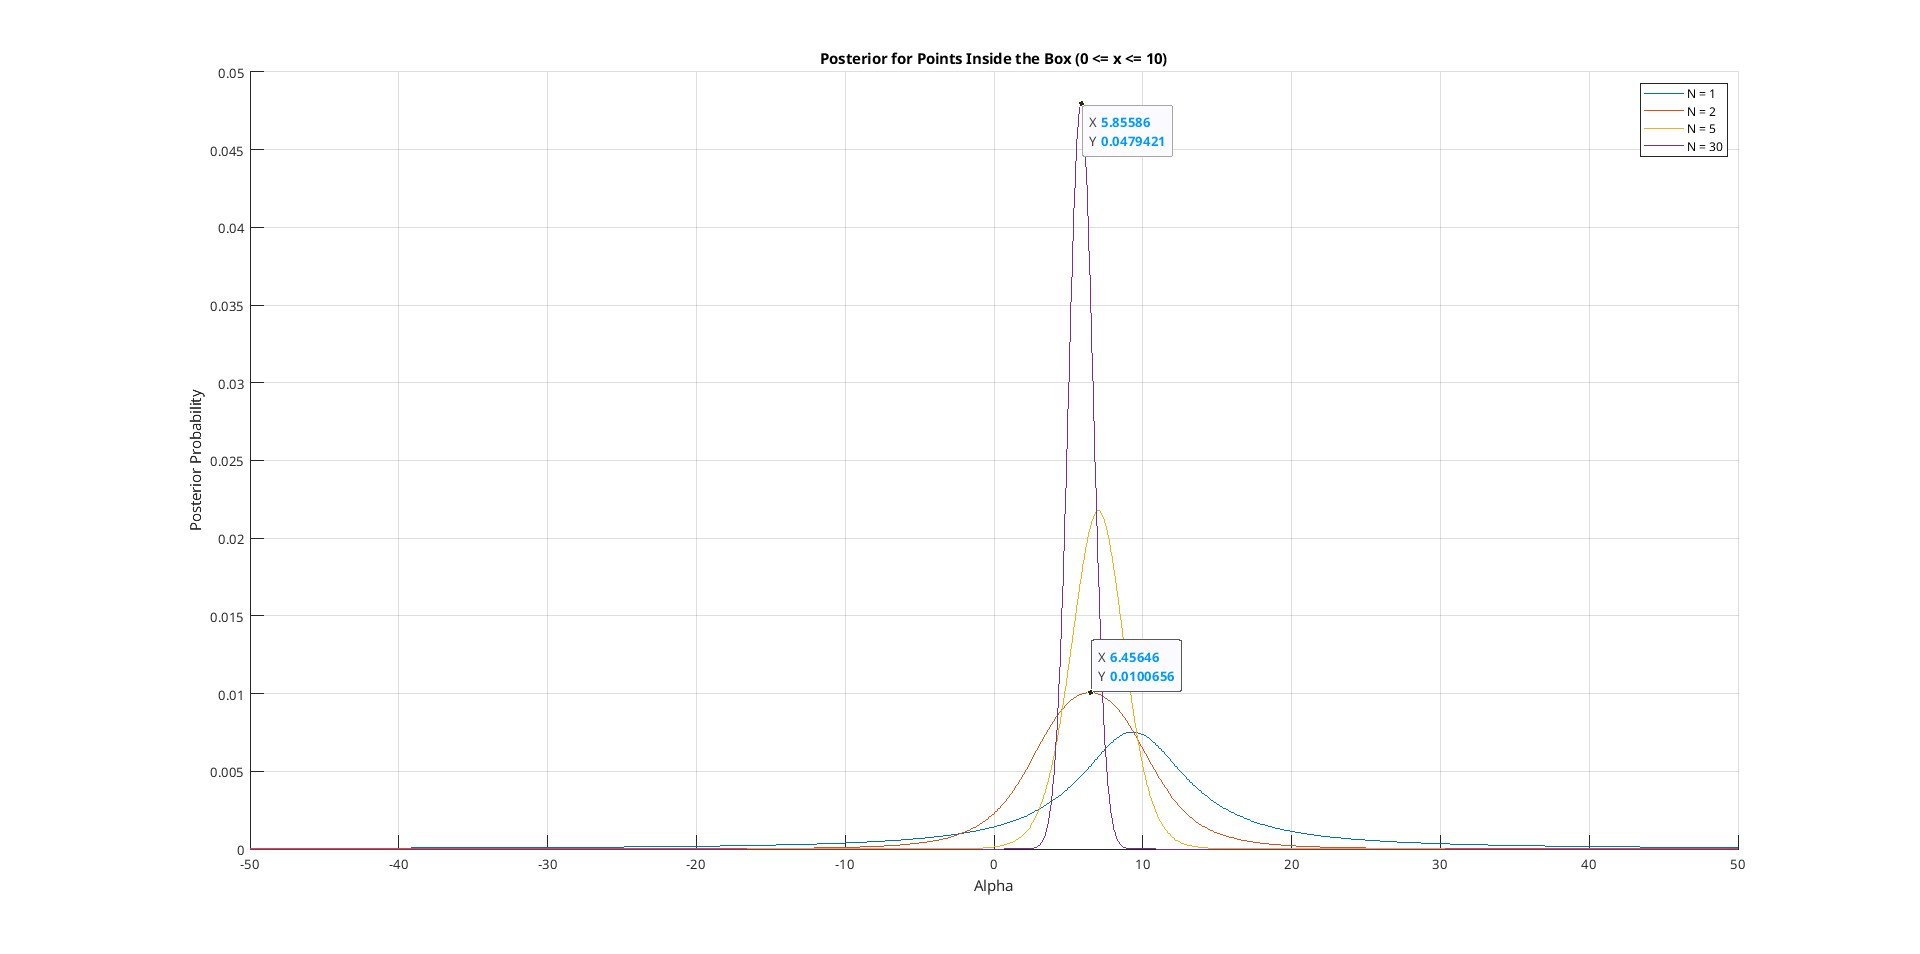
\includegraphics[scale=0.2]{q07pdfinbox.jpg} 
        \caption{Bayes' Inference Scheme Plot of the PDF for points inside the box}
\end{figure}	

\begin{figure}[h]
        \centering
        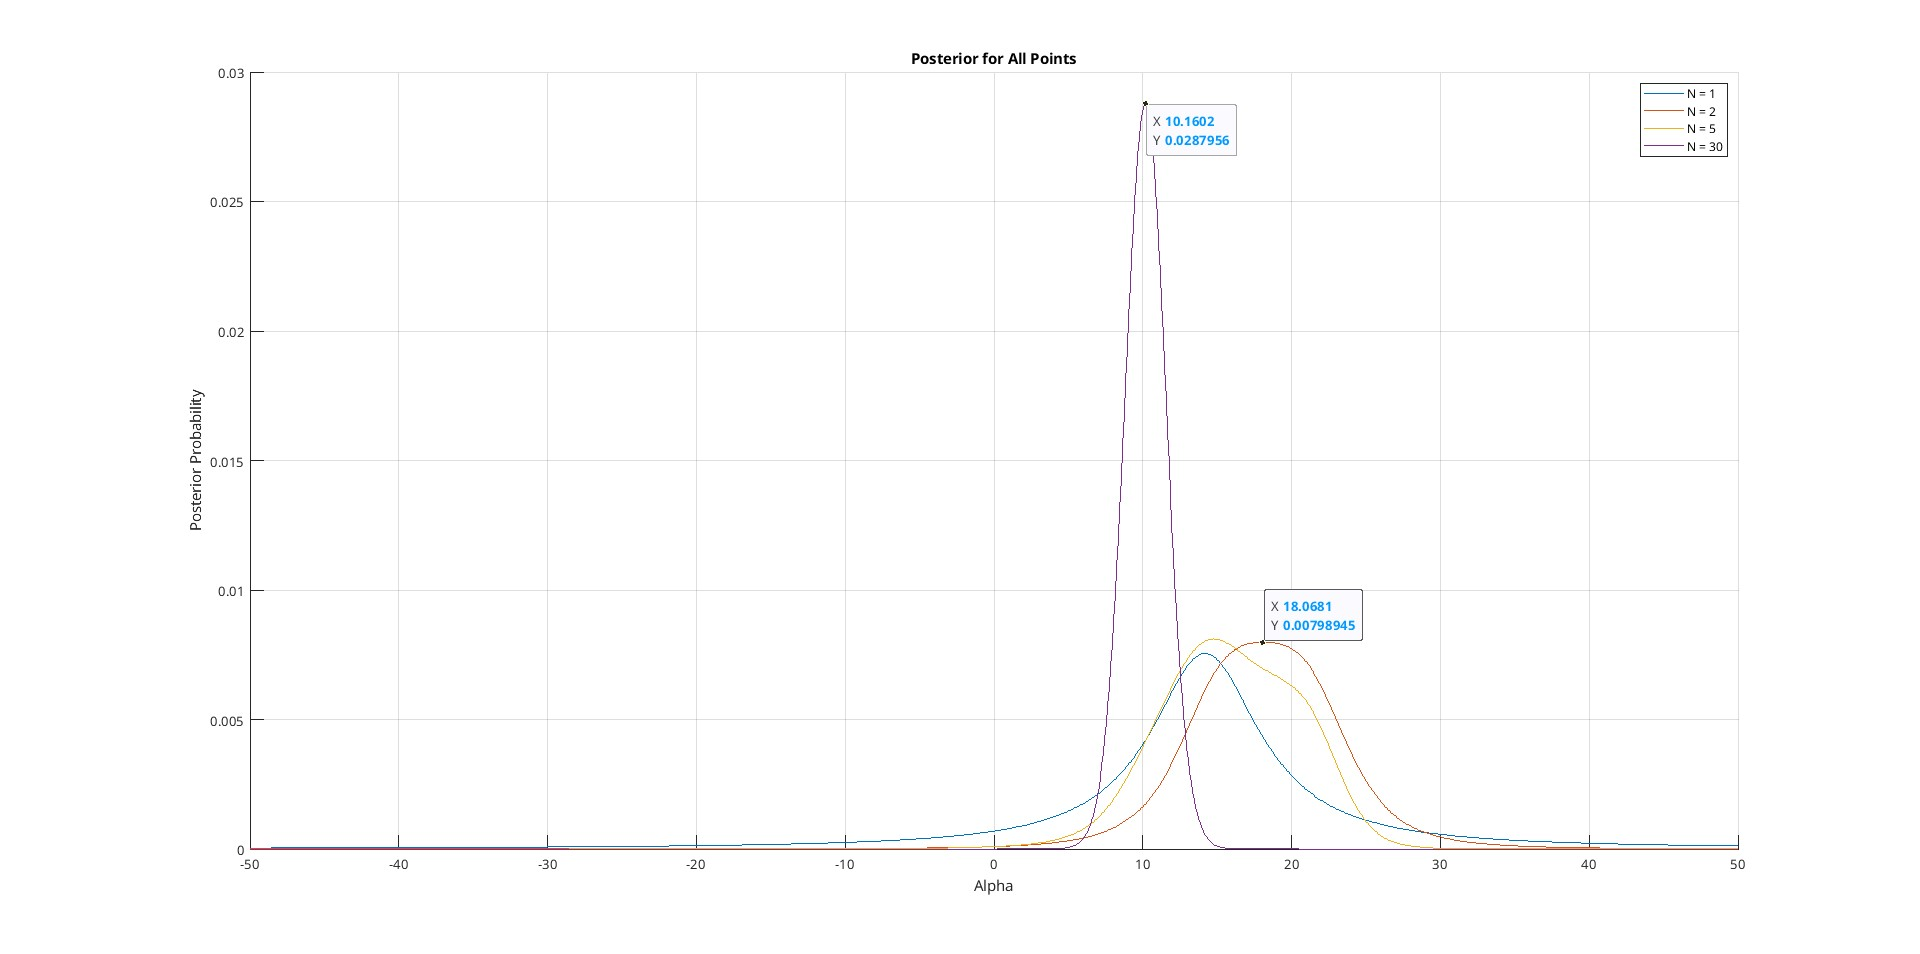
\includegraphics[scale=0.2]{q07pdfoutbox.jpg} 
        \caption{Bayes' Inference Scheme Plot of the PDF for all points}
\end{figure}	

\newpage
\section{Appendix C. - Maximum Likelyhood Estimation Scheme}
\begin{lstlisting}[language=Matlab,
                   numbers=left,
                   basicstyle=\small,
                   stepnumber=1,
                   numbersep=10pt,
                   tabsize=2,
                   showspaces=false,
                   showstringspaces=false]
%%%%%%%%%Estimating alpha using Maximum Likelyhood Solution%%%%%%%%%%%%
%numbat24.04%
%
load('BayesData.mat');

% Given y-position
beta = 4.5;

% Define the log-likelihood function so that product becomes a sum
log_likelihood = @(alpha) sum(log(beta ./ (pi * (beta^2 + (x - alpha).^2))));

% Find the alpha that maximizes the log-likelihood, 
% use fminsearch to minimize the negative log-likelihood, (equivalent to
% maximizing the likelihood)
alpha_mle = fminsearch(@(alpha) -log_likelihood(alpha), mean(x));

% Display the MLE result
disp(['Maximum Likelihood Estimate for alpha: ', num2str(alpha_mle)]);
%% alpha = 7.2287 %%
\end{lstlisting}

\end{document}
